\documentclass{templatebeamerufc/libs/ufc_format}
% Inserting the preamble file with the packages
\input{templatebeamerufc/libs/preamble.tex}
%%% Local Variables:
%%% mode: latex
%%% TeX-master: t
%%% End:

% macros de utilidade
\newcommand{\fonteautor}{Elaborado pelo autor.}
\newcommand{\fonteautorscikit}{Elaborado pelo autor baseado nas
  imagens disponíveis em~\citeonline{scikit-image}.}
\newcommand{\red}[1]{\textcolor{red}{\textbf{#1}}}  % bold red text

\listfiles
% Title
\title[EGSIS]{\textbf{Segmentação Semi-Supervisionada de Imagens através de
Dinâmicas Coletivas em Redes Complexas}}
% Subtitle
\subtitle{Uma avaliação no cenário de segmentação interativa}
% Author of the presentation
\author{Manoel Vilela Machado Neto}
% Institute's Name
\institute[UFC]{
    % email for contact
    \normalsize{\email{manoel.machado@alu.ufc.br}}
    \newline
    % Department Name
    \department{Engenharia da Computação}
    \newline
    % university name
    \ufc{}
}
% date of the presentation
\date{Sobral, \today}


%%%%%%%%%%%%%%%%%%%%%%%%%%%%%%%%%%%%%%%%%%%%%%%%%%%%%%%%%%%%%%%%%%%%%%%%%%%%%%%%%%
%% Start Document of the Presentation                                           %%
%%%%%%%%%%%%%%%%%%%%%%%%%%%%%%%%%%%%%%%%%%%%%%%%%%%%%%%%%%%%%%%%%%%%%%%%%%%%%%%%%%
\begin{document}
% insert the code style
\input{templatebeamerufc/libs/code_style}
%% ---------------------------------------------------------------------------
% First frame (with tile, subtitle, ...)
\begin{frame}{}
    \maketitle
\end{frame}

%% ---------------------------------------------------------------------------
% Second frame
\begin{frame}[allowframebreaks]{Sumário}
  \tableofcontents[sections={1-2}]
    \framebreak{}
  \tableofcontents[sections={3-5}]
\end{frame}

%% ---------------------------------------------------------------------------
% This presentation is separated by sections and subsections
\section{Introdução}

%% ---------------------------------------------------------------------------
\subsection{Tipos de segmentação de imagem}

\begin{frame}{Definição do problema}
  \begin{block}{Definição}
      Em segmentação de imagens, o objetivo é dividir imagens em regiões
      de interesse.
  \end{block}

  Existem alguns tipos diferentes de segmentação de imagens, como por
exemplo:
  \begin{enumerate}
    \item Segmentação semântica;
    \item Segmentação de instâncias;
    \item Segmentação interativa.
  \end{enumerate}
\end{frame}


\begin{frame}{Segmentação de instâncias e semântica}
  % imagem comparando segmentação semântica vs segmentação por instâncias
  \begin{figure}\label{fig:semantic-vs-instance-segmentation}
    \centering
    \caption{Comparação entre segmentação semântica e segmentação de instâncias.}
    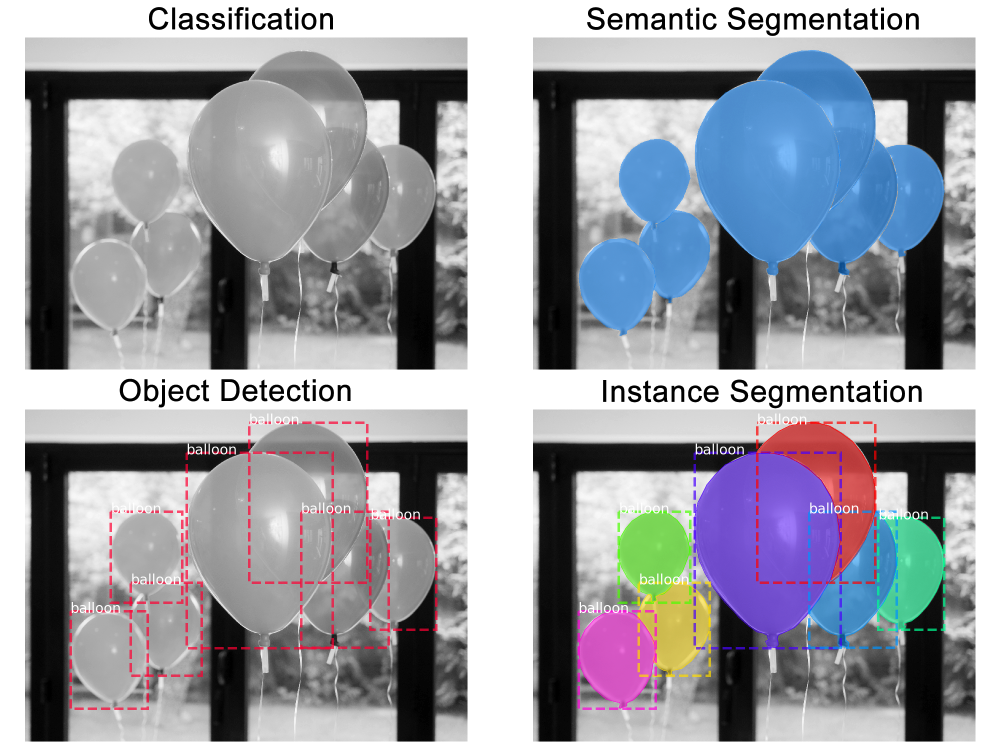
\includegraphics[scale=0.2]{figuras/image-segmentation-types}
    \source{\cite{MediumInstanceSegmentation2019}}
  \end{figure}
\end{frame}

\begin{frame}{Segmentação interativa}
  \begin{figure}\label{fig:interactive--segmentation}
    \centering
    \caption{Ilustração de segmentação interativa, rotulação em azul e
      vermelho.\\ Na imagem a direita, foto segmentada.}
    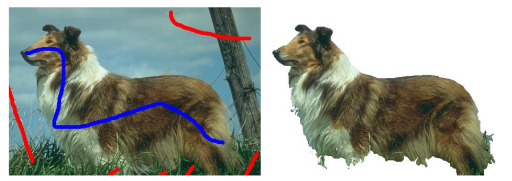
\includegraphics[scale=0.6]{figuras/interactive-segmentation-2008}
    \source{\cite{duchenne2008segmentation}}
  \end{figure}
\end{frame}



%% ---------------------------------------------------------------------------
\subsection{Aprendizagem semi-supervisionada}
\subsection{Algoritmos indutivos vs transdutivos}
\begin{frame}{Criando Caixas}
    \successbox{testando o success box}

    \pause

    \alertbox{testando o alert box}

    \pause

    \simplebox{testando o simple box}
\end{frame}

\section{Fundamentação Teórica}
\subsection{Superpixels}
\subsection{Redes complexas}
\subsection{Extração de características}
\subsection{Dinâmicas coletivas}
\subsection{EGSIS}
\begin{frame}{Seção II - Multicolunas}
    \begin{columns}{}
        \begin{column}{0.5\textwidth}
            \justify
            É possível colocar mais de uma coluna utilizando os comandos de $\backslash$begin\{column\}\{\} e $\backslash$end\{column\}
        \end{column}
        \begin{column}{0.5\textwidth}
            \justify
            Porém, o espaçamento deve ser proporcional entre as colunas para que estas colunas não entrem em coflito. O espaçamento é dado pelo segundo argumento do $\backslash$begin.
        \end{column}
    \end{columns}
\end{frame}


% This frame show an example to insert multicolumns

\section{Metodologia}
\begin{frame}{Seção II - Multicolunas}
    \begin{columns}{}
        \begin{column}{0.5\textwidth}
            \justify
            É possível colocar mais de uma coluna utilizando os comandos de $\backslash$begin\{column\}\{\} e $\backslash$end\{column\}
        \end{column}
        \begin{column}{0.5\textwidth}
            \justify
            Porém, o espaçamento deve ser proporcional entre as colunas para que estas colunas não entrem em coflito. O espaçamento é dado pelo segundo argumento do $\backslash$begin.
        \end{column}
    \end{columns}
\end{frame}

\subsection{Dataset GrabCut}

\subsection{Métricas de avaliação}


\section{Resultados}

\subsection{Variação na quantidade de superpixels}
\subsection{Resultados qualitativos}
\subsection{Resultados quantitativos}

\section{Conclusão}
\begin{frame}{Seção II - Multicolunas}
    \begin{columns}{}
        \begin{column}{0.5\textwidth}
            \justify
            É possível colocar mais de uma coluna utilizando os comandos de $\backslash$begin\{column\}\{\} e $\backslash$end\{column\}
        \end{column}
        \begin{column}{0.5\textwidth}
            \justify
            Porém, o espaçamento deve ser proporcional entre as colunas para que estas colunas não entrem em coflito. O espaçamento é dado pelo segundo argumento do $\backslash$begin.
        \end{column}
    \end{columns}
\end{frame}

\subsection{Limitações e desafios}
\subsection{Trabalhos futuros}


%% ---------------------------------------------------------------------------
% Reference frames
\begin{frame}[allowframebreaks]
  \frametitle{Referências}
  % Inserting the references file
  \bibliography{3-pos-textuais/referencias.bib}
  %\printbibliography{}
\end{frame}

%% ---------------------------------------------------------------------------
% Final frame
\begin{frame}{}
    \centering
    \huge{\textbf{\example{Obrigado pela atenção!}}}

    \vspace{1cm}

    \Large{\textbf{Contato:}}
    \newline
    \vspace*{0.5cm}
    \large{\email{manoel.machado@alu.ufc.br}}
\end{frame}

\end{document}
